\documentclass[11pt]{article}
\newcommand\tab[1][1cm]{\hspace*{#1}}
\usepackage{graphicx}
\graphicspath{ {C:/Users/yedkk/Desktop/CS465/hw4} }
\begin{document}
\section{Homework 9}
Name: Kangdong Yuan
	
\subsection{problem1}
a).I did not work in a group.
\\b).I did not consult without anyone my group members
\\c).I did not consult any non-class materials.

\subsection{problem2}
We prove by contradiction.\\
Given $e^*$ is the heaviest edge in some cycle C of undirected graph G.\\
We assume the claim is Flase, so T is a minimal spanning forest and $e^* \in T$. Let $S, \ V-S$ be the two connected components in $T \setminus \{e\}$. Since C is a cycle, there are two edges in C that cut $S, \ V-S$. We define another edge is r. The $e^*$ has more cost than edge r, which is $w(e)>w(r)$. So, the new minimal spanning forest with edge r cost less than minimal spanning forest with edge $e^*$. It is a contradiction to the minimal cost principle of minimal spanning forest.\\
So, $e^*$ cannot in minimal spanning forest, which cannot appear in any MST of G.


\subsection{problem3}
a). $f_a>f_b \ and \ f_a>f_c$, so $f_a=10, f_b=5, f_c=5$\\
b). This encoding is not possible, because the code for $a$ is $(0)$, is a prefix of the code for $c$ is $(00)$. \\
c). This encoding is not optimal, because the $\{0,10,11\}$ cost less space. And, the Huffman tree of this encoding is not complete, which is not optimal. 

\subsection{problem4}
we can construct Huffman tree to find prefix-free encoding of minimal total cost.
As a common convention, bit '0' represents following the left child and bit '1' represents following the right child.\\
\\
First, using a priority queue $Q$ to store all the words as key and $f_i*c_i$ as value. In Q, lowest value is given highest priority. \\
\\
1. Create a leaf node for each symbol and add it to the	Q.\\
2. While there is more than one node in the queue:\\
\tab Remove the two nodes from Q (lowest $f_i*c_i$)\\
\tab Create a new internal node with these two nodes as children and with value ($f_i*c_i$) equal to the sum of the two nodes' value ($f_i*c_i$).\\
\tab Add the new node to the queue.\\
3. The remaining node is the root node and the tree is complete.\\

Then the prefix-free encoding of each word is path of each node. for example\\
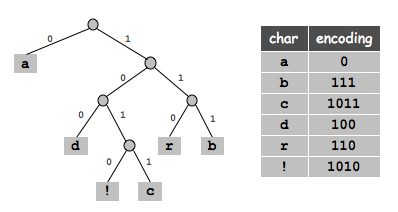
\includegraphics[scale=0.7]{huff}\\
Time complexity: $O(nlogn)$, because each iteration requires $O(logn)$ time to determine the lowest frequencies and insert the new word in priority queue. There are $O(n)$ iterations.





\end{document}